\documentclass{article}
\usepackage{amsmath, tikz, tcolorbox, array, sfmath, enumerate, pgfplots, marvosym, amssymb, multicol}
\renewcommand{\familydefault}{\sfdefault}
\pgfplotsset{compat=newest}
\usepgfplotslibrary{fillbetween}
% \everymath{\displaystyle}
\tikzset{>=stealth}
\usepackage[top = 0.25in, bottom = 0.25in, left = 1.25in, right = 1.25in]{geometry}
\pagestyle{empty}
\raggedright

\tikzset{>=stealth}
\tikzstyle{input} = [circle, text centered, radius = 1cm, draw = black]
\tikzstyle{function} = [rectangle, text centered, minimum width = 2cm, minimum height = 1cm, draw = black]

\newcounter{example}[section]
\newenvironment{example}[1][]{\refstepcounter{example}\par\medskip
   {\color{red}\textbf{Example~\theexample. #1}}}{\medskip}

\begin{document}

\section*{Functions}

\begin{tcolorbox}[colframe=orange!70!white, coltitle=black, title=\textbf{Summary}]
\begin{enumerate}
    \item Functions take a single input value and produce a single output value.
    \item Interval notation can be used in place of inequalities.
    \item When finding domain, you can't divide by 0 or take the square root of a negative number.
\end{enumerate}
\end{tcolorbox}
\vspace{1in}

Think of a function as a \textbf{machine}. 
\vspace{0.5in}

You give the function (machine) a value (input), \newline 
it will process that value, and then return a value back to you (output).
\vspace{1in}

For instance, if you input 10 into the $x^2$ function, it will return $10^2$, or 100:	\newline\\

\begin{center}
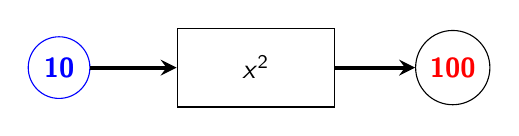
\begin{tikzpicture}[node distance = 2.5 cm]
\node (inputVal) [input, color=blue] {\color{blue}\textbf{10}};
\node (func) [function, right of = inputVal] {$x^2$};
\node (outputVal) [input, right of = func] {\color{red}\textbf{100}};

\draw [->, >=stealth, thick, line width = 1.5] (inputVal) -- (func);
\draw [->, >=stealth, thick, line width = 1.5] (func) -- (outputVal);
\end{tikzpicture}
\end{center}
\vfill 

A function can be described using \textbf{function notation}. 
\vfill 
$f(x)$ represents the value of the function when the value of $x$ is substituted into it.
\vfill 
We can use other notations for functions including, but not limited to,
\[ g(x) \quad h(x) \quad f(n) \quad f\left(\text{\Smiley}\right) \]
\vfill 

When we substitute a value for the variable and evaluate it, that is called {\color{blue}\textbf{evaluating the function}}.
\vfill 
\newpage

\begin{example}
Evaluate $f(2), \, f(-2), \, \text{and } f(0)$ for each.
\begin{enumerate}[(a)]
    \item $f(x) = 2x + 3$   \vfill 
    \item $f(x) = 3x^2-1$   \vfill 
    \item \mbox{} \newline\\
    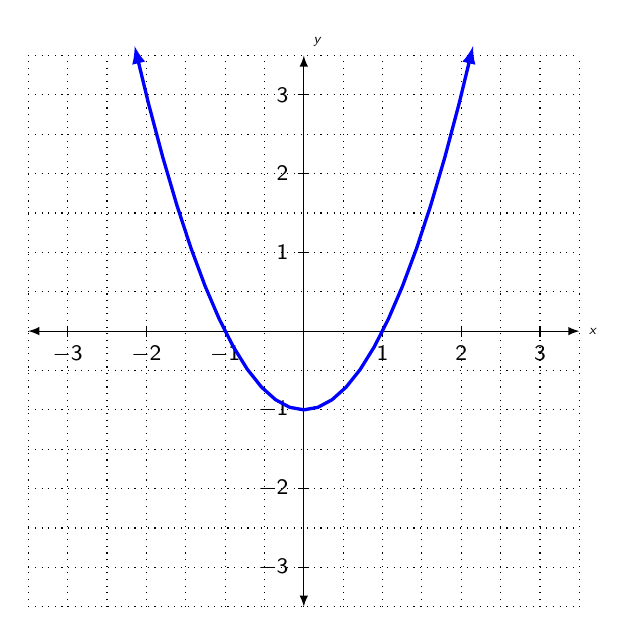
\begin{tikzpicture}[domain = -2.15:2.15]
	\draw [step = 0.5cm, dotted] (-3.5,-3.5) grid (3.5,3.5);
	\draw[<->, > = latex] (-3.5,0) -- (3.5,0);
	\node at (3.5,0) [anchor = west] {\tiny $x$};
	\draw[<->, > = latex] (0,-3.5) -- (0,3.5);
	\node at (0,3.5) [anchor = south west] {\tiny $y$};
	\foreach \x in {-3,-2,-1,1,2,3}
	\draw[shift = {(\x,0)}] (0pt,2pt) -- (0pt, -2pt) node[below] {\footnotesize $\x$};
	\foreach \y in {-3,-2, -1, 1, 2, 3}
	\draw[shift = {(0,\y)}] (2pt,0pt) -- (-2pt,0pt) node[left] {\footnotesize $\y$};
	\draw [<->, > = latex, color = blue, very thick]	plot (\x, {\x*\x - 1});
    \end{tikzpicture}
    \vfill 
    \item \mbox{} \newline\\
    \begin{tabular}{|c|c|c|c|c|c|c|c|}
        $x$ & $-3$ & $-2$ & $-1$ & 0 & 1 & 2 & 3 \\ \hline
        $f(x)$ & $-6$ & 3 & 4 & $-3$ & $-8$ & 6 & $-5$ \\
    \end{tabular}
    \vfill 
\end{enumerate}
\end{example}

\newpage 


\subsection*{Interval Notation}
\vspace{0.5in}

We often use interval notation to denote the domain and range of a function.
\vspace{0.5in}

\begin{center}
\setlength{\extrarowheight}{8pt}
\scalebox{0.9}{
\begin{tabular}{|c|c|c|}
\hline \textbf{Interval Notation} & \textbf{Set-Builder Notation} & \textbf{Graph} \\[5pt] 
\hline 
$(4, \, 9)$ & $\lbrace x \mid 4<x<9 \rbrace$ & 
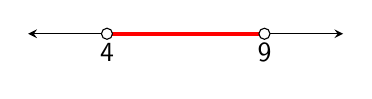
\begin{tikzpicture}[baseline=(current bounding box.north)]
    \coordinate (A) at (0,0);
    \coordinate (B) at (2,0);
    \draw [<->, >=stealth] (-1,0) -- (3,0);
    \node at (A) [anchor = north] {$4$};
    \node at (B) [anchor = north] {$9$};
    \draw [red, ultra thick] (A) -- (B);
    \draw [fill=white] (A) circle (2pt);
    \draw [fill=white] (B) circle (2pt);
\end{tikzpicture}
\\
\hline $[4, \, 9]$ & $\lbrace x \mid 4\leq x \leq 9 \rbrace$ & 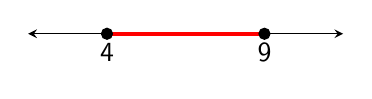
\begin{tikzpicture}[baseline=(current bounding box.north)]
    \coordinate (A) at (0,0);
    \coordinate (B) at (2,0);
    \draw [<->, >=stealth] (-1,0) -- (3,0);
    \node at (A) [anchor = north] {$4$};
    \node at (B) [anchor = north] {$9$};
    \draw [red, ultra thick] (A) -- (B);
    \draw [fill=black] (A) circle (2pt);
    \draw [fill=black] (B) circle (2pt);
\end{tikzpicture}
\\
\hline $[4, \, 9)$ & $\lbrace x \mid 4 \leq x < 9 \rbrace$ & 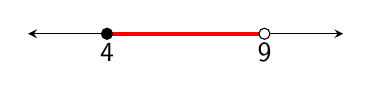
\begin{tikzpicture}[baseline=(current bounding box.north)]
    \coordinate (A) at (0,0);
    \coordinate (B) at (2,0);
    \draw [<->, >=stealth] (-1,0) -- (3,0);
    \node at (A) [anchor = north] {$4$};
    \node at (B) [anchor = north] {$9$};
    \draw [red, ultra thick] (A) -- (B);
    \draw [fill=black] (A) circle (2pt);
    \draw [fill=white] (B) circle (2pt);
\end{tikzpicture} 
\\
\hline $(4, \, 9]$ & $\lbrace x \mid 4 < x \leq 9 \rbrace$ & 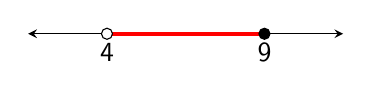
\begin{tikzpicture}[baseline=(current bounding box.north)]
    \coordinate (A) at (0,0);
    \coordinate (B) at (2,0);
    \draw [<->, >=stealth] (-1,0) -- (3,0);
    \node at (A) [anchor = north] {$4$};
    \node at (B) [anchor = north] {$9$};
    \draw [red, ultra thick] (A) -- (B);
    \draw [fill=white] (A) circle (2pt);
    \draw [fill=black] (B) circle (2pt);
\end{tikzpicture} 
\\[0.15in]  
\hline $(4, \, \infty)$ & $\lbrace x \mid x > 4 \rbrace$ & 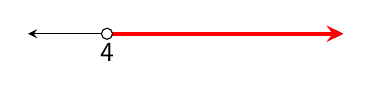
\begin{tikzpicture}[baseline=(current bounding box.north)]
    \coordinate (A) at (0,0);
    \coordinate (B) at (2,0);
    \draw [<->, >=stealth] (-1,0) -- (3,0);
    \node at (A) [anchor = north] {$4$};
    \draw [red, ultra thick, ->, >=stealth] (A) -- (3,0);
    \draw [fill=white] (A) circle (2pt);
\end{tikzpicture} 
\\

\hline $[4, \, \infty)$ & $\lbrace x \mid x \geq 4 \rbrace$ & 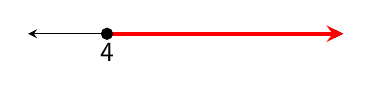
\begin{tikzpicture}[baseline=(current bounding box.north)]
    \coordinate (A) at (0,0);
    \coordinate (B) at (2,0);
    \draw [<->, >=stealth] (-1,0) -- (3,0);
    \node at (A) [anchor = north] {$4$};
    \draw [red, ultra thick, ->, >=stealth] (A) -- (3,0);
    \draw [fill=black] (A) circle (2pt);
\end{tikzpicture} 
\\

\hline $(-\infty, \, 9)$ & $\lbrace x \mid x < 9 \rbrace$ & 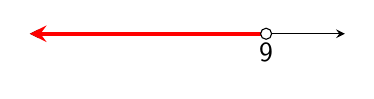
\begin{tikzpicture}[baseline=(current bounding box.north)]
    \coordinate (A) at (0,0);
    \coordinate (B) at (2,0);
    \draw [<->, >=stealth] (-1,0) -- (3,0);
    \node at (B) [anchor = north] {$9$};
    \draw [red, ultra thick, ->, >=stealth] (B) -- (-1,0);
    \draw [fill=white] (B) circle (2pt);
\end{tikzpicture} 
\\

\hline $(-\infty, \, 9]$ & $\lbrace x \mid x \leq 9 \rbrace$ & 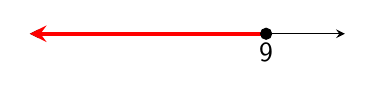
\begin{tikzpicture}[baseline=(current bounding box.north)]
    \coordinate (A) at (0,0);
    \coordinate (B) at (2,0);
    \draw [<->, >=stealth] (-1,0) -- (3,0);
    \node at (B) [anchor = north] {$9$};
    \draw [red, ultra thick, ->, >=stealth] (B) -- (-1,0);
    \draw [fill=black] (B) circle (2pt);
\end{tikzpicture} 
\\[0.15in]  
\hline $(-\infty, \, \infty)$ & $\mathbb{R}$ & 
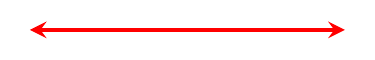
\begin{tikzpicture}[baseline=(current bounding box.north)]
    \draw [<->, >=stealth, red, ultra thick] (-1,0) -- (3,0);
\end{tikzpicture} 
\\[0.15in]

\hline  $\varnothing$   & $\{ \, \}$ & 
\begin{tikzpicture}[baseline=(current bounding box.north)]
    \draw [<->, >=stealth] (-1,0) -- (3,0);
\end{tikzpicture} 
\\[0.15in]  \hline
\end{tabular}}
\end{center}

\vfill 

\subsection*{Domain of a Function}
\vspace{0.25in}

The {\color{blue}\textbf{domain}} of a function is the set of all possible \emph{input} values that we are allowed to plug in to a function. \newline\\

The {\color{violet}\textbf{range}} of a function is the set of all possible \emph{output} values that we get from the function. \newline\\

\textsc{2 Domain Issues:}
\begin{itemize}
    \item Can't divide by 0. \quad $\dfrac{}{\neq 0}$ \newline\\
    \item Can't take the square root of a negative number. \quad $\sqrt{\geq 0}$
\end{itemize}

\vfill 
\newpage 

\begin{example}
Determine the domain of each. Write your answer using interval notation.
\begin{enumerate}[(a)]
    \item $f(x) = \sqrt{5x-2}$  \vspace{2.5in}
    \item $g(x) = \frac{3}{x^2-4x}$
\end{enumerate}
\end{example}


\end{document}
